\section*{Funkce}

\subsection*{Značení}

\begin{table}[H]
    \centering
    \begin{tabular}{c|c}
        značení & co se tím myslí \\
        \hline
        $[a,b]$ & uzavřený interval v mezích $a$ a $b$\\
        $\N$ & množina přirozených čísel \\
        $\Z$ & množina celých čísel \\
        $\R$ & množina reálných čísel
    \end{tabular}
\end{table}

\subsection*{Základní pojmy}

\textbf{Funkcí} obecně rozumíme zobrazení z nějaké množiny $A$ do reálných čísel $\R$. To znamená, že nějakým prvkům z množiny $A$ přiřazujeme reálná čísla. Symbolicky to zapisujeme jako \begin{align}
    f: A \to \R \:.
\end{align}

\begin{itemize}
    \item Funkce $f: \R \to \R$ je reálná funkce jedné reálné proměnné. Zapisujeme ji ve tvaru $f(x)$, kde $x$ je nezávislá proměnná.
    \item Funkce $a: \N \to \R$ je posloupnost reálných čísel, přiřazuje hodnoty číslům $1,2,3, \cdots$. Namísto $a(n)$ píšeme $a_n$, čímž naznačujeme, že indexy probíhají přirozená čísla. (Posloupnostem se budeme věnovat od poloviny semestru.)
    \item Funkce $F: \R \times \R \to \R$ přiřazuje dvěma reálným číslům jiné reálné číslo, hovoříme o funkci dvou proměnných. Zapisujeme ji ve tvaru $F(x,y)$, kde $x$ a $y$ jsou nezávislé proměnné. (Funkce dvou proměnných potkáme v poslední čtvrtině semestru.) 
\end{itemize}

Nezávislé proměnné $x$ ve funkci $f(x)$ také někdy říkáme \textbf{argument funkce}, závislé proměnné $f(x_0)$ říkáme \textbf{funkční hodnota v bodě $x_0$}.


\textbf{Definiční obor} $D(f)$, $D_f$ je množina takových čísel, pro která je funkce definována. \textbf{Obor hodnot} $H(f)$, $H_f$, $R_f$ je množina všech možných funkčních hodnot dané funkce. 

\subsection*{Elementární funkce}

Elementární funkce jsou takové, které lze složit konečným počtem operací (sčítání, odčítání, násobení, dělení a skládání) z těchto funkcí: konstanta, obecná mocnina, exponenciála, logaritmus, sinus, kosinus, tangens, kotangens, arkussinus, arkuskosinus, arkustangens a arkuskotangens. 

Jiné funkce než elementární v kurzu prakticky nepotkáme. Je jich ale spousta. Příklady neelementárních funkcí si ukážeme, až budeme vybaveni mocnými nástroji, jako je určitý integrál.

\subsection*{Prostá funkce, inverzní funkce}

Označíme-li $f(x) = y$, můžeme se ptát na otázku, zda bychom mohli zpětně dopočítat argument funkce $x$ při znalosti $y$. Pokud to lze, můžeme vytvořit \textbf{inverzní funkci} $f^{-1}(x)$ danou vztahem $f^{-1}(y) = x$.

\begin{example}[Lineární funkce]
    K funkci $f(x) = 3x-6$ můžeme najít inverzní. Označíme si $3x-6=y$ a pokusíme se vyjádřit $x$. Zřejmě $x = \frac{1}{3}(y+6)$. Předpis pro inverzní funkci tedy bude $f^{-1}(x) = \frac{1}{3} (x+6)$.
\end{example}

\begin{example}[Potíže s kvadratickou funkcí]
    Pokusíme-li se hledat inverzní funkci k $f(x) = x^2$, narazíme na problém. Jedné hodnotě $y$ příslušejí dvě různé hodnoty, a to sice $\sqrt{y}$ anebo $-\sqrt{y}$. Například pokud položíme $y = 16$, pak máme možnosti $x=4$ anebo $x=-4$. Vidíme, že na celé množině $\R$ nemůžeme inverzní funkci stanovit, protože potřebujeme jednoznačnost.
\end{example}

Předchozí příklad nás vede k podmínce, kterou musí daná funkce splňovat, abychom k ní mohli sestrojit inverzní. Řekneme, že funkce $f$ je \textbf{prostá} na intervalu $I$, jestliže \begin{align}
    x_1, x_2 \in I : x_1 \neq x_2 \implies f(x_1) \neq f(x_2) \:.
\end{align}
Slovně řečeno: vybereme-li si dvě různá $x$, nesmí se rovnat jejich funkční hodnoty $f(x)$.

Definiční obor a obor hodnot se u inverzní funkce prohazují: \begin{align}
    D_{f^{-1}} = H_f \:, \quad H_{f^{-1}} = D_f \:.
\end{align}

Graf funkce $f^{-1}$ lze získat z grafu $f$ tak, že jej nakreslíme osově symetricky podle přímky $y=x$.


\begin{example}[Odstranění potíží]
    Funkce z předchozího příkladu $f(x) = x^2$ je prostá na intervalu $[0,\infty)$, tam k ní existuje inverzní funkce $f^{-1}(x)=\sqrt{x}$, a na intervalu $(-\infty,0]$, tam k ní existuje inverzní funkce $f^{-1}(x)=-\sqrt{x}$.

    \begin{figure}[H]
        \centering
        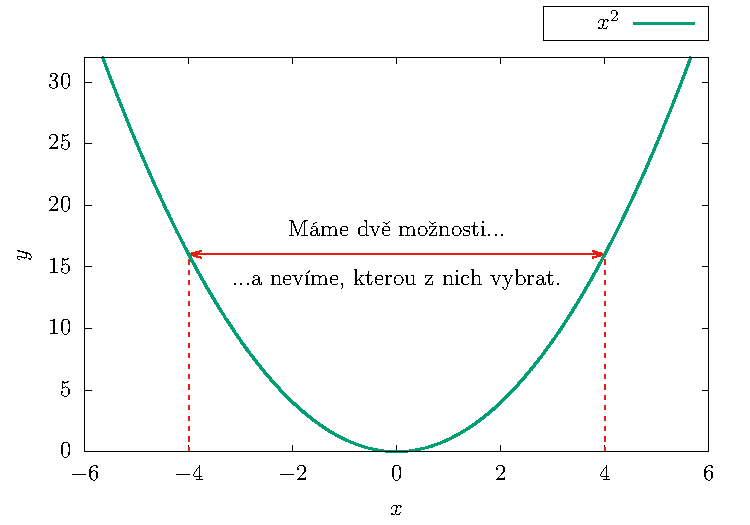
\includegraphics[scale = 0.7]{Gnuplot/cv1/Figures/nejednoznacny.pdf}
        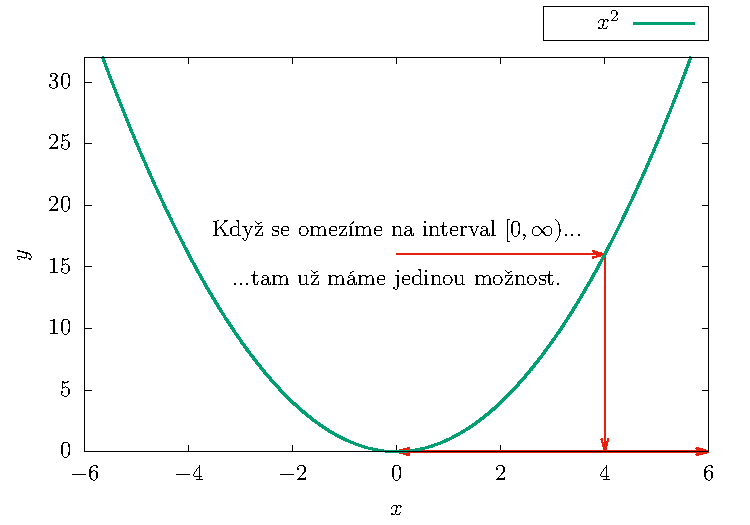
\includegraphics[scale = 0.7]{Gnuplot/cv1/Figures/nejednoznacny-reseni.pdf}
    \end{figure}

\end{example}

\begin{example}[Exponenciální funkce, přirozený logaritmus]
    Definujeme exponenciální funkci $\exp(x) = e^x$, kde $e = 2,718281828\cdots$ je tzv. Eulerovo číslo. (Je iracionální, stejně jako číslo $\pi$, číslice v desetinném zápisu se neopakují.) Dále definujeme funkci k ní inverzní - přirozený logaritmus $\ln(x) = \log_e (x)$. 
    Platí \begin{align}
        D(\exp(x)) = \R \:,\quad H(\exp(x)) = (0,+\infty) \:,\quad  D(\ln(x)) = (0,+\infty) \:,\quad  H(\ln(x)) = \R \:.
    \end{align}
    Užitečné vztahy, které se vyplatí pamatovat, jsou: \begin{align}
        e^0 = 1 \:,&\quad \ln(1) =0 \\
        e^{x+y} = e^x e^y \:,& \quad e^{ax} = (e^x)^a\\
        \ln(xy) = \ln x + \ln y \:,& \quad \ln(x^a) = a \ln x 
    \end{align}
    Grafy obou funkcí jsou znázorněny na obrázku \ref{fig:exp-log}.

    \begin{figure}[H]
        \centering
        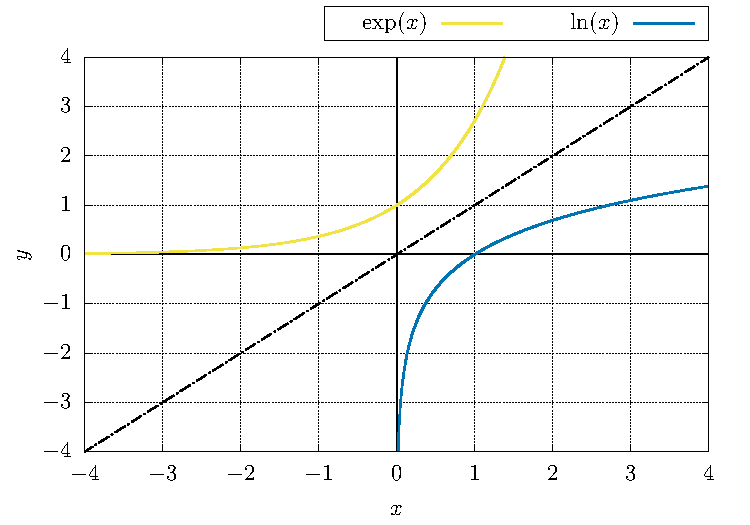
\includegraphics{Gnuplot/cv1/Figures/exp-log.pdf}
        \caption{Grafy funkcí exponenciály a přirozeného logaritmu. Všimněme si, že jsou grafy navzájem osově symetrické podle přímky $y=x$.}
        \label{fig:exp-log}
    \end{figure}

\end{example}